% Dr. E. Lasker - J. R. Capablanca, St. Petersburg, 1914, with Capablanca's notes.
% Build with: python3 ../../tools/chessbook.py game-05-lasker-capablanca.tex
\documentclass[10pt,twoside]{article}
\usepackage[paperwidth=487.56bp,paperheight=691.65bp,top=72pt,bottom=44pt,inner=50pt,outer=48pt,
            headheight=13pt,headsep=20pt,footskip=0pt]{geometry}
\usepackage[T1]{fontenc}
\usepackage[lining]{ebgaramond}
\usepackage{graphicx}
\usepackage{microtype}
\usepackage{tikz}
\usepackage{fancyhdr}
\usepackage[hidelinks,pdftitle={Lasker - Capablanca, St. Petersburg, 1914},
            pdfauthor={J. R. Capablanca}]{hyperref}

\newcommand{\textsizebook}{\fontsize{10.5}{12.6}\selectfont}
\AtBeginDocument{\textsizebook}
\setlength{\columnsep}{11pt}
\setlength{\parindent}{9pt}
\setlength{\parskip}{0pt}
\setlength{\emergencystretch}{1.5em}
\raggedbottom

\newlength{\boardwidth}
\setlength{\boardwidth}{160pt}

% A main line move, as a bold heading above its note
\newcommand{\Move}[1]{\par\addvspace{8pt}\noindent\phantomsection{\bfseries #1}\par\nopagebreak}
% A diagram in the text
\newcommand{\ChessDiagram}[1]{\par\addvspace{7pt}{\centering #1\par}\addvspace{5pt}}

\pagestyle{fancy}
\fancyhf{}
\renewcommand{\headrulewidth}{0pt}
\fancyhead[LE,RO]{\thepage}
\fancyhead[CE]{Ruy Lopez}
\fancyhead[CO]{Lasker -- Capablanca}






\newcommand{\figK}{\raisebox{-0.14em}{
\includegraphics[height=1em]{diagrams/figK}}}
\newcommand{\figQ}{\raisebox{-0.14em}{
\includegraphics[height=1em]{diagrams/figQ}}}
\newcommand{\figR}{\raisebox{-0.14em}{
\includegraphics[height=1em]{diagrams/figR}}}
\newcommand{\figB}{\raisebox{-0.14em}{
\includegraphics[height=1em]{diagrams/figB}}}
\newcommand{\figN}{\raisebox{-0.14em}{
\includegraphics[height=1em]{diagrams/figN}}}
\begin{document}

\twocolumn[{%
\thispagestyle{empty}
\begin{tikzpicture}[remember picture,overlay]
  \node[circle,draw=black,line width=1.6pt,fill=black!20,minimum size=112pt] (seal)
       at ([xshift=75pt,yshift=-75pt]current page.north west) {};
  \draw[line width=0.9pt] ([shift={(-48pt,-30pt)}]seal.center) -- ([shift={(44pt,34pt)}]seal.center);
  \node[rotate=37] at ([shift={(-11pt,14pt)}]seal.center) {\fontsize{25}{25}\selectfont\bfseries Game};
  \node[rotate=37] at ([shift={(10pt,-16pt)}]seal.center) {\fontsize{38}{38}\selectfont\bfseries 5};
  \node[anchor=north east] at ([xshift=-14pt,yshift=-24pt]current page.north east)
       {\href{https://lichess.org/analysis/pgn/e4_e5_Nf3_Nc6_Bb5_a6_Bxc6_dxc6}{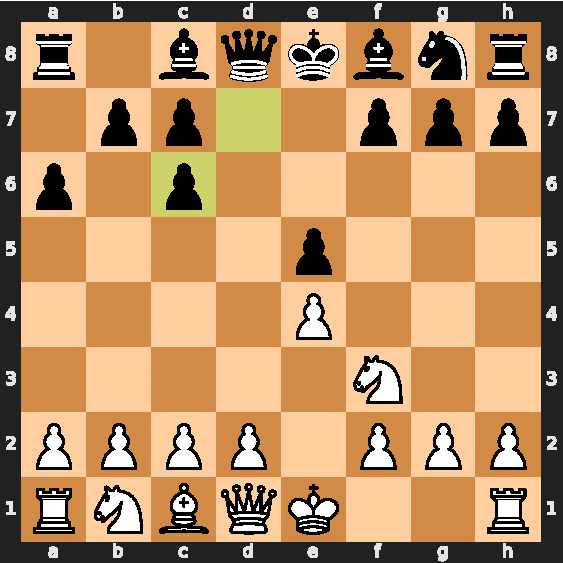
\includegraphics[width=108pt]{diagrams/board-8e9ff290c4c2}}};
\end{tikzpicture}

\vspace*{38pt}
\begin{center}
  \begin{minipage}{235pt}\centering
    {\fontsize{22}{25}\selectfont\bfseries Ruy Lopez\par}
    \vspace{4pt}\rule{\linewidth}{1pt}\\[-9.5pt]\rule{\linewidth}{0.4pt}
  \end{minipage}

  \vspace{14pt}
  {\fontsize{19}{22}\selectfont\bfseries Lasker -- Capablanca\par}
  \vspace{10pt}
  {\fontsize{15}{18}\selectfont\bfseries St. Petersburg, 1914\par}
  \vspace{8pt}
  {\fontsize{11}{13}\selectfont White: Dr. E. Lasker \quad Black: J. R. Capablanca\par}
  \vspace{10pt}
  {\centering\fontsize{8.5}{10}\selectfont\itshape
   Notes by J. R. Capablanca, from \textup{Chess Fundamentals} (1921), which is in the public domain.\\
   Descriptive notation has been converted to algebraic. Page references are to the book.\\
   Click any move or diagram to open it on Lichess.\par}
\end{center}
\vspace{10pt}
}]
\textsizebook

\Move{\href{https://lichess.org/analysis/pgn/e4}{1.e4} \href{https://lichess.org/analysis/pgn/e4_e5}{e5} \href{https://lichess.org/analysis/pgn/e4_e5_Nf3}{2.\figN f3} \href{https://lichess.org/analysis/pgn/e4_e5_Nf3_Nc6}{\figN c6} \href{https://lichess.org/analysis/pgn/e4_e5_Nf3_Nc6_Bb5}{3.\figB b5} \href{https://lichess.org/analysis/pgn/e4_e5_Nf3_Nc6_Bb5_a6}{a6} \href{https://lichess.org/analysis/pgn/e4_e5_Nf3_Nc6_Bb5_a6_Bxc6}{4.\figB xc6}}

The object of this move is to bring about speedily a middle-game without Queens, in which White has four Pawns to three on the King's side, while Black's superiority of Pawns on the other side is somewhat balanced by the fact that one of Black's Pawns is doubled. On the other hand, Black has the advantage of remaining with two Bishops while White has only one.

\Move{\href{https://lichess.org/analysis/pgn/e4_e5_Nf3_Nc6_Bb5_a6_Bxc6_dxc6}{4...dxc6} \href{https://lichess.org/analysis/pgn/e4_e5_Nf3_Nc6_Bb5_a6_Bxc6_dxc6_d4}{5.d4} \href{https://lichess.org/analysis/pgn/e4_e5_Nf3_Nc6_Bb5_a6_Bxc6_dxc6_d4_exd4}{exd4} \href{https://lichess.org/analysis/pgn/e4_e5_Nf3_Nc6_Bb5_a6_Bxc6_dxc6_d4_exd4_Qxd4}{6.\figQ xd4} \href{https://lichess.org/analysis/pgn/e4_e5_Nf3_Nc6_Bb5_a6_Bxc6_dxc6_d4_exd4_Qxd4_Qxd4}{\figQ xd4} \href{https://lichess.org/analysis/pgn/e4_e5_Nf3_Nc6_Bb5_a6_Bxc6_dxc6_d4_exd4_Qxd4_Qxd4_Nxd4}{7.\figN xd4} \href{https://lichess.org/analysis/pgn/e4_e5_Nf3_Nc6_Bb5_a6_Bxc6_dxc6_d4_exd4_Qxd4_Qxd4_Nxd4_Bd6}{\figB d6}}

Black's idea is to Castle on the King's side. His reason is that the King ought to remain on the weaker side to oppose later the advance of White's Pawns. Theoretically there is very much to be said in favour of this reasoning, but whether in practice that would be the best system would be rather difficult to prove. The student should notice that if now all the pieces were exchanged White would practically be a Pawn ahead, and would therefore have a won ending.

\Move{\href{https://lichess.org/analysis/pgn/e4_e5_Nf3_Nc6_Bb5_a6_Bxc6_dxc6_d4_exd4_Qxd4_Qxd4_Nxd4_Bd6_Nc3}{8.\figN c3} \href{https://lichess.org/analysis/pgn/e4_e5_Nf3_Nc6_Bb5_a6_Bxc6_dxc6_d4_exd4_Qxd4_Qxd4_Nxd4_Bd6_Nc3_Ne7}{\figN e7}}

A perfectly sound form of development. In any other form adopted the Black Knight could not be developed either as quickly or as well. e7 is the natural position for the Black Knight in this variation, in order not to obstruct Black's Pawns, and also, in some eventualities, in order to go to g6. There is also the possibility of its going to d4 via c6 after ...c5.

\Move{\href{https://lichess.org/analysis/pgn/e4_e5_Nf3_Nc6_Bb5_a6_Bxc6_dxc6_d4_exd4_Qxd4_Qxd4_Nxd4_Bd6_Nc3_Ne7_O-O}{9.0--0} \href{https://lichess.org/analysis/pgn/e4_e5_Nf3_Nc6_Bb5_a6_Bxc6_dxc6_d4_exd4_Qxd4_Qxd4_Nxd4_Bd6_Nc3_Ne7_O-O_O-O}{0--0} \href{https://lichess.org/analysis/pgn/e4_e5_Nf3_Nc6_Bb5_a6_Bxc6_dxc6_d4_exd4_Qxd4_Qxd4_Nxd4_Bd6_Nc3_Ne7_O-O_O-O_f4}{10.f4}}

This move I considered weak at the time, and I do still. It leaves the e-pawn weak, unless it advances to e5, and it also makes it possible for Black to pin the Knight by \figB c5.

\Move{\href{https://lichess.org/analysis/pgn/e4_e5_Nf3_Nc6_Bb5_a6_Bxc6_dxc6_d4_exd4_Qxd4_Qxd4_Nxd4_Bd6_Nc3_Ne7_O-O_O-O_f4_Re8}{10...\figR e8}}

Best. It threatens \figB c5; \figB e3, \figN d5. It also prevents \figB e3 because of \figN d5 or f5.

\Move{\href{https://lichess.org/analysis/pgn/e4_e5_Nf3_Nc6_Bb5_a6_Bxc6_dxc6_d4_exd4_Qxd4_Qxd4_Nxd4_Bd6_Nc3_Ne7_O-O_O-O_f4_Re8_Nb3}{11.\figN b3} \href{https://lichess.org/analysis/pgn/e4_e5_Nf3_Nc6_Bb5_a6_Bxc6_dxc6_d4_exd4_Qxd4_Qxd4_Nxd4_Bd6_Nc3_Ne7_O-O_O-O_f4_Re8_Nb3_f6}{f6}}

Preparatory to ...b6, followed by ...c5 and \figB b7 in conjunction with \figN g6, which would put White in great difficulties to meet the combined attack against the two centre Pawns.

\Move{\href{https://lichess.org/analysis/pgn/e4_e5_Nf3_Nc6_Bb5_a6_Bxc6_dxc6_d4_exd4_Qxd4_Qxd4_Nxd4_Bd6_Nc3_Ne7_O-O_O-O_f4_Re8_Nb3_f6_f5}{12.f5}}

\ChessDiagram{\href{https://lichess.org/analysis/pgn/e4_e5_Nf3_Nc6_Bb5_a6_Bxc6_dxc6_d4_exd4_Qxd4_Qxd4_Nxd4_Bd6_Nc3_Ne7_O-O_O-O_f4_Re8_Nb3_f6_f5}{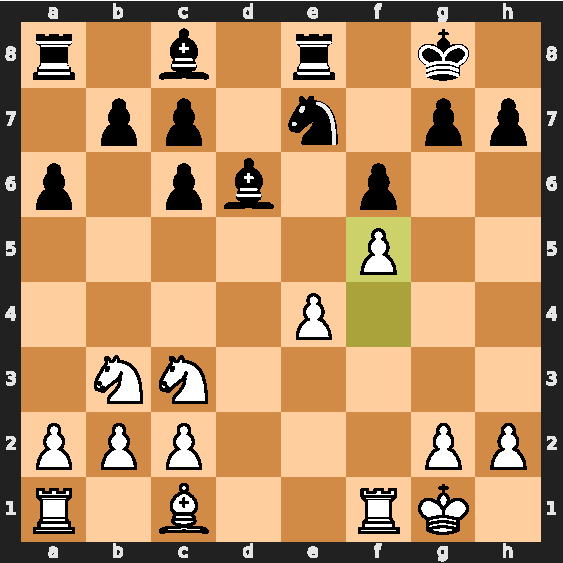
\includegraphics[width=\boardwidth]{diagrams/board-b1b66d0fac22}}}

It has been wrongly claimed that this wins the game, but I would like nothing better than to have such a position again. It required several mistakes on my part finally to obtain a lost position.

\Move{\href{https://lichess.org/analysis/pgn/e4_e5_Nf3_Nc6_Bb5_a6_Bxc6_dxc6_d4_exd4_Qxd4_Qxd4_Nxd4_Bd6_Nc3_Ne7_O-O_O-O_f4_Re8_Nb3_f6_f5_b6}{12...b6} \href{https://lichess.org/analysis/pgn/e4_e5_Nf3_Nc6_Bb5_a6_Bxc6_dxc6_d4_exd4_Qxd4_Qxd4_Nxd4_Bd6_Nc3_Ne7_O-O_O-O_f4_Re8_Nb3_f6_f5_b6_Bf4}{13.\figB f4}}

\ChessDiagram{\href{https://lichess.org/analysis/pgn/e4_e5_Nf3_Nc6_Bb5_a6_Bxc6_dxc6_d4_exd4_Qxd4_Qxd4_Nxd4_Bd6_Nc3_Ne7_O-O_O-O_f4_Re8_Nb3_f6_f5_b6_Bf4}{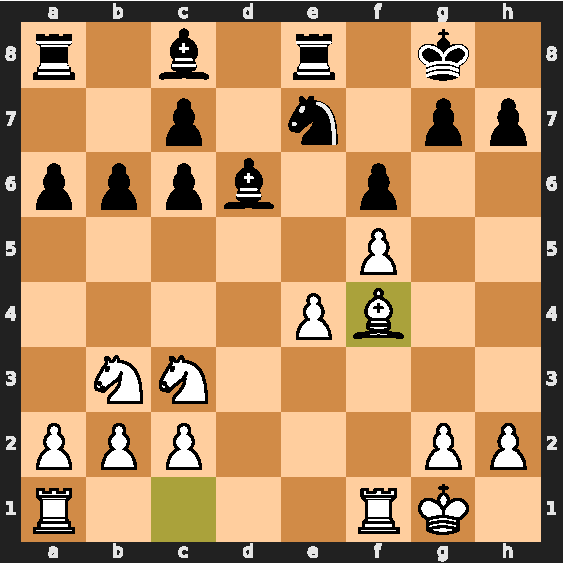
\includegraphics[width=\boardwidth]{diagrams/board-988eea2c5485}}}

\Move{\href{https://lichess.org/analysis/pgn/e4_e5_Nf3_Nc6_Bb5_a6_Bxc6_dxc6_d4_exd4_Qxd4_Qxd4_Nxd4_Bd6_Nc3_Ne7_O-O_O-O_f4_Re8_Nb3_f6_f5_b6_Bf4_Bb7}{13...\figB b7}}

Played against my better judgment. The right move of course was \href{https://lichess.org/analysis/pgn/e4_e5_Nf3_Nc6_Bb5_a6_Bxc6_dxc6_d4_exd4_Qxd4_Qxd4_Nxd4_Bd6_Nc3_Ne7_O-O_O-O_f4_Re8_Nb3_f6_f5_b6_Bf4_Bxf4}{13...\figB xf4}. Dr. Lasker gives the following variation: \href{https://lichess.org/analysis/pgn/e4_e5_Nf3_Nc6_Bb5_a6_Bxc6_dxc6_d4_exd4_Qxd4_Qxd4_Nxd4_Bd6_Nc3_Ne7_O-O_O-O_f4_Re8_Nb3_f6_f5_b6_Bf4_Bxf4}{13...\figB xf4} \href{https://lichess.org/analysis/pgn/e4_e5_Nf3_Nc6_Bb5_a6_Bxc6_dxc6_d4_exd4_Qxd4_Qxd4_Nxd4_Bd6_Nc3_Ne7_O-O_O-O_f4_Re8_Nb3_f6_f5_b6_Bf4_Bxf4_Rxf4}{14.\figR xf4} \href{https://lichess.org/analysis/pgn/e4_e5_Nf3_Nc6_Bb5_a6_Bxc6_dxc6_d4_exd4_Qxd4_Qxd4_Nxd4_Bd6_Nc3_Ne7_O-O_O-O_f4_Re8_Nb3_f6_f5_b6_Bf4_Bxf4_Rxf4_c5}{c5} \href{https://lichess.org/analysis/pgn/e4_e5_Nf3_Nc6_Bb5_a6_Bxc6_dxc6_d4_exd4_Qxd4_Qxd4_Nxd4_Bd6_Nc3_Ne7_O-O_O-O_f4_Re8_Nb3_f6_f5_b6_Bf4_Bxf4_Rxf4_c5_Rd1}{15.\figR d1} \href{https://lichess.org/analysis/pgn/e4_e5_Nf3_Nc6_Bb5_a6_Bxc6_dxc6_d4_exd4_Qxd4_Qxd4_Nxd4_Bd6_Nc3_Ne7_O-O_O-O_f4_Re8_Nb3_f6_f5_b6_Bf4_Bxf4_Rxf4_c5_Rd1_Bb7}{\figB b7} \href{https://lichess.org/analysis/pgn/e4_e5_Nf3_Nc6_Bb5_a6_Bxc6_dxc6_d4_exd4_Qxd4_Qxd4_Nxd4_Bd6_Nc3_Ne7_O-O_O-O_f4_Re8_Nb3_f6_f5_b6_Bf4_Bxf4_Rxf4_c5_Rd1_Bb7_Rf2}{16.\figR f2} \href{https://lichess.org/analysis/pgn/e4_e5_Nf3_Nc6_Bb5_a6_Bxc6_dxc6_d4_exd4_Qxd4_Qxd4_Nxd4_Bd6_Nc3_Ne7_O-O_O-O_f4_Re8_Nb3_f6_f5_b6_Bf4_Bxf4_Rxf4_c5_Rd1_Bb7_Rf2_Rad8}{\figR ad8} \href{https://lichess.org/analysis/pgn/e4_e5_Nf3_Nc6_Bb5_a6_Bxc6_dxc6_d4_exd4_Qxd4_Qxd4_Nxd4_Bd6_Nc3_Ne7_O-O_O-O_f4_Re8_Nb3_f6_f5_b6_Bf4_Bxf4_Rxf4_c5_Rd1_Bb7_Rf2_Rad8_Rxd8}{17.\figR xd8} \href{https://lichess.org/analysis/pgn/e4_e5_Nf3_Nc6_Bb5_a6_Bxc6_dxc6_d4_exd4_Qxd4_Qxd4_Nxd4_Bd6_Nc3_Ne7_O-O_O-O_f4_Re8_Nb3_f6_f5_b6_Bf4_Bxf4_Rxf4_c5_Rd1_Bb7_Rf2_Rad8_Rxd8_Rxd8}{\figR xd8} \href{https://lichess.org/analysis/pgn/e4_e5_Nf3_Nc6_Bb5_a6_Bxc6_dxc6_d4_exd4_Qxd4_Qxd4_Nxd4_Bd6_Nc3_Ne7_O-O_O-O_f4_Re8_Nb3_f6_f5_b6_Bf4_Bxf4_Rxf4_c5_Rd1_Bb7_Rf2_Rad8_Rxd8_Rxd8_Rd2}{18.\figR d2} \href{https://lichess.org/analysis/pgn/e4_e5_Nf3_Nc6_Bb5_a6_Bxc6_dxc6_d4_exd4_Qxd4_Qxd4_Nxd4_Bd6_Nc3_Ne7_O-O_O-O_f4_Re8_Nb3_f6_f5_b6_Bf4_Bxf4_Rxf4_c5_Rd1_Bb7_Rf2_Rad8_Rxd8_Rxd8_Rd2_Rxd2}{\figR xd2} \href{https://lichess.org/analysis/pgn/e4_e5_Nf3_Nc6_Bb5_a6_Bxc6_dxc6_d4_exd4_Qxd4_Qxd4_Nxd4_Bd6_Nc3_Ne7_O-O_O-O_f4_Re8_Nb3_f6_f5_b6_Bf4_Bxf4_Rxf4_c5_Rd1_Bb7_Rf2_Rad8_Rxd8_Rxd8_Rd2_Rxd2_Nxd2}{19.\figN xd2}, and he claims that White has the best of it. But, as Niemzovitch pointed out immediately after the game, \href{https://lichess.org/analysis/pgn/e4_e5_Nf3_Nc6_Bb5_a6_Bxc6_dxc6_d4_exd4_Qxd4_Qxd4_Nxd4_Bd6_Nc3_Ne7_O-O_O-O_f4_Re8_Nb3_f6_f5_b6_Bf4_Bxf4_Rxf4_c5_Rd1_Bb7_Rf2_Rad8}{16...\figR ad8} given in Dr. Lasker's variation, is not the best. If \href{https://lichess.org/analysis/pgn/e4_e5_Nf3_Nc6_Bb5_a6_Bxc6_dxc6_d4_exd4_Qxd4_Qxd4_Nxd4_Bd6_Nc3_Ne7_O-O_O-O_f4_Re8_Nb3_f6_f5_b6_Bf4_Bxf4_Rxf4_c5_Rd1_Bb7_Rf2_Rac8}{16...\figR ac8!} then White will have great difficulty in drawing the game, since there is no good way to stop Black from playing \figN c6, followed by \figN e5, threatening \figN c4. And should White attempt to meet this manoeuvre by withdrawing the Knight at b3; then the Black Knight can go to d4, and the White Pawn at e4 will be the object of the attack. Taking Dr. Lasker's variation, however, whatever advantage there might be disappears at once if Black plays \href{https://lichess.org/analysis/pgn/e4_e5_Nf3_Nc6_Bb5_a6_Bxc6_dxc6_d4_exd4_Qxd4_Qxd4_Nxd4_Bd6_Nc3_Ne7_O-O_O-O_f4_Re8_Nb3_f6_f5_b6_Bf4_Bxf4_Rxf4_c5_Rd1_Bb7_Rf2_Rad8_Rxd8_Rxd8_Rd2_Rxd2_Nxd2_Nc6}{19...\figN c6}, threatening \figN b4 and also \figN d4, neither of which can be stopped. If White answers \href{https://lichess.org/analysis/pgn/e4_e5_Nf3_Nc6_Bb5_a6_Bxc6_dxc6_d4_exd4_Qxd4_Qxd4_Nxd4_Bd6_Nc3_Ne7_O-O_O-O_f4_Re8_Nb3_f6_f5_b6_Bf4_Bxf4_Rxf4_c5_Rd1_Bb7_Rf2_Rad8_Rxd8_Rxd8_Rd2_Rxd2_Nxd2_Nc6_Nd5}{20.\figN d5} \href{https://lichess.org/analysis/pgn/e4_e5_Nf3_Nc6_Bb5_a6_Bxc6_dxc6_d4_exd4_Qxd4_Qxd4_Nxd4_Bd6_Nc3_Ne7_O-O_O-O_f4_Re8_Nb3_f6_f5_b6_Bf4_Bxf4_Rxf4_c5_Rd1_Bb7_Rf2_Rad8_Rxd8_Rxd8_Rd2_Rxd2_Nxd2_Nc6_Nd5_Nd4}{\figN d4} for Black will at least draw. In fact, after \href{https://lichess.org/analysis/pgn/e4_e5_Nf3_Nc6_Bb5_a6_Bxc6_dxc6_d4_exd4_Qxd4_Qxd4_Nxd4_Bd6_Nc3_Ne7_O-O_O-O_f4_Re8_Nb3_f6_f5_b6_Bf4_Bxf4_Rxf4_c5_Rd1_Bb7_Rf2_Rad8_Rxd8_Rxd8_Rd2_Rxd2_Nxd2_Nc6}{19...\figN c6} Black threatens so many things that it is difficult to see how White can prevent the loss of one or more Pawns.

\Move{\href{https://lichess.org/analysis/pgn/e4_e5_Nf3_Nc6_Bb5_a6_Bxc6_dxc6_d4_exd4_Qxd4_Qxd4_Nxd4_Bd6_Nc3_Ne7_O-O_O-O_f4_Re8_Nb3_f6_f5_b6_Bf4_Bb7_Bxd6}{14.\figB xd6} \href{https://lichess.org/analysis/pgn/e4_e5_Nf3_Nc6_Bb5_a6_Bxc6_dxc6_d4_exd4_Qxd4_Qxd4_Nxd4_Bd6_Nc3_Ne7_O-O_O-O_f4_Re8_Nb3_f6_f5_b6_Bf4_Bb7_Bxd6_cxd6}{cxd6} \href{https://lichess.org/analysis/pgn/e4_e5_Nf3_Nc6_Bb5_a6_Bxc6_dxc6_d4_exd4_Qxd4_Qxd4_Nxd4_Bd6_Nc3_Ne7_O-O_O-O_f4_Re8_Nb3_f6_f5_b6_Bf4_Bb7_Bxd6_cxd6_Nd4}{15.\figN d4}}

It is a curious but true fact that I did not see this move when I played \href{https://lichess.org/analysis/pgn/e4_e5_Nf3_Nc6_Bb5_a6_Bxc6_dxc6_d4_exd4_Qxd4_Qxd4_Nxd4_Bd6_Nc3_Ne7_O-O_O-O_f4_Re8_Nb3_f6_f5_b6_Bf4_Bb7}{13...\figB b7}, otherwise I would have played the right move \href{https://lichess.org/analysis/pgn/e4_e5_Nf3_Nc6_Bb5_a6_Bxc6_dxc6_d4_exd4_Qxd4_Qxd4_Nxd4_Bd6_Nc3_Ne7_O-O_O-O_f4_Re8_Nb3_f6_f5_b6_Bf4_Bxf4}{13...\figB xf4}.

\Move{\href{https://lichess.org/analysis/pgn/e4_e5_Nf3_Nc6_Bb5_a6_Bxc6_dxc6_d4_exd4_Qxd4_Qxd4_Nxd4_Bd6_Nc3_Ne7_O-O_O-O_f4_Re8_Nb3_f6_f5_b6_Bf4_Bb7_Bxd6_cxd6_Nd4_Rad8}{15...\figR ad8}}

The game is yet far from lost, as against the entry of the Knight, Black can later on play ...c5, followed by ...d5.

\Move{\href{https://lichess.org/analysis/pgn/e4_e5_Nf3_Nc6_Bb5_a6_Bxc6_dxc6_d4_exd4_Qxd4_Qxd4_Nxd4_Bd6_Nc3_Ne7_O-O_O-O_f4_Re8_Nb3_f6_f5_b6_Bf4_Bb7_Bxd6_cxd6_Nd4_Rad8_Ne6}{16.\figN e6} \href{https://lichess.org/analysis/pgn/e4_e5_Nf3_Nc6_Bb5_a6_Bxc6_dxc6_d4_exd4_Qxd4_Qxd4_Nxd4_Bd6_Nc3_Ne7_O-O_O-O_f4_Re8_Nb3_f6_f5_b6_Bf4_Bb7_Bxd6_cxd6_Nd4_Rad8_Ne6_Rd7}{\figR d7} \href{https://lichess.org/analysis/pgn/e4_e5_Nf3_Nc6_Bb5_a6_Bxc6_dxc6_d4_exd4_Qxd4_Qxd4_Nxd4_Bd6_Nc3_Ne7_O-O_O-O_f4_Re8_Nb3_f6_f5_b6_Bf4_Bb7_Bxd6_cxd6_Nd4_Rad8_Ne6_Rd7_Rad1}{17.\figR ad1}}

\ChessDiagram{\href{https://lichess.org/analysis/pgn/e4_e5_Nf3_Nc6_Bb5_a6_Bxc6_dxc6_d4_exd4_Qxd4_Qxd4_Nxd4_Bd6_Nc3_Ne7_O-O_O-O_f4_Re8_Nb3_f6_f5_b6_Bf4_Bb7_Bxd6_cxd6_Nd4_Rad8_Ne6_Rd7_Rad1}{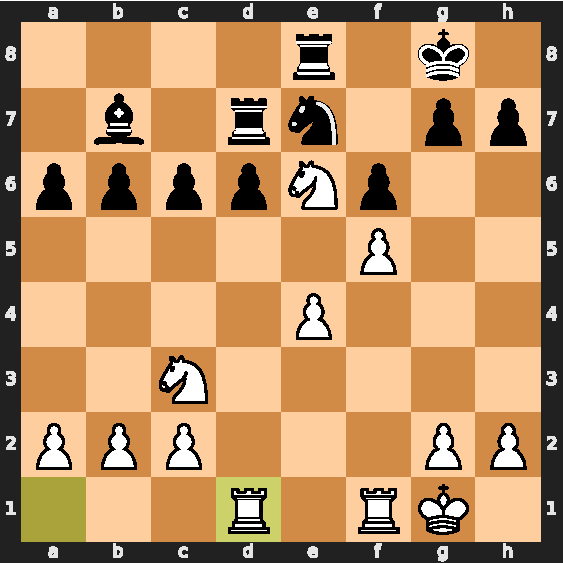
\includegraphics[width=\boardwidth]{diagrams/board-6b3433b5e06a}}}

I now was on the point of playing ...c5, to be followed by ...d5, which I thought would give me a draw, but suddenly I became ambitious and thought that I could play the text move, \href{https://lichess.org/analysis/pgn/e4_e5_Nf3_Nc6_Bb5_a6_Bxc6_dxc6_d4_exd4_Qxd4_Qxd4_Nxd4_Bd6_Nc3_Ne7_O-O_O-O_f4_Re8_Nb3_f6_f5_b6_Bf4_Bb7_Bxd6_cxd6_Nd4_Rad8_Ne6_Rd7_Rad1_Nc8}{17...\figN c8}, and later on sacrifice the exchange for the Knight at e6, winning a Pawn for it, and leaving White's e-pawn still weaker. I intended to carry this plan either before or after playing ...g5 as the circumstances demanded. Now let us analyse: \href{https://lichess.org/analysis/pgn/e4_e5_Nf3_Nc6_Bb5_a6_Bxc6_dxc6_d4_exd4_Qxd4_Qxd4_Nxd4_Bd6_Nc3_Ne7_O-O_O-O_f4_Re8_Nb3_f6_f5_b6_Bf4_Bb7_Bxd6_cxd6_Nd4_Rad8_Ne6_Rd7_Rad1_c5}{17...c5}. If \href{https://lichess.org/analysis/pgn/e4_e5_Nf3_Nc6_Bb5_a6_Bxc6_dxc6_d4_exd4_Qxd4_Qxd4_Nxd4_Bd6_Nc3_Ne7_O-O_O-O_f4_Re8_Nb3_f6_f5_b6_Bf4_Bb7_Bxd6_cxd6_Nd4_Rad8_Ne6_Rd7_Rad1_c5_Nd5}{18.\figN d5} \href{https://lichess.org/analysis/pgn/e4_e5_Nf3_Nc6_Bb5_a6_Bxc6_dxc6_d4_exd4_Qxd4_Qxd4_Nxd4_Bd6_Nc3_Ne7_O-O_O-O_f4_Re8_Nb3_f6_f5_b6_Bf4_Bb7_Bxd6_cxd6_Nd4_Rad8_Ne6_Rd7_Rad1_c5_Nd5_Bxd5}{\figB xd5} \href{https://lichess.org/analysis/pgn/e4_e5_Nf3_Nc6_Bb5_a6_Bxc6_dxc6_d4_exd4_Qxd4_Qxd4_Nxd4_Bd6_Nc3_Ne7_O-O_O-O_f4_Re8_Nb3_f6_f5_b6_Bf4_Bb7_Bxd6_cxd6_Nd4_Rad8_Ne6_Rd7_Rad1_c5_Nd5_Bxd5_exd5}{19.exd5} \href{https://lichess.org/analysis/pgn/e4_e5_Nf3_Nc6_Bb5_a6_Bxc6_dxc6_d4_exd4_Qxd4_Qxd4_Nxd4_Bd6_Nc3_Ne7_O-O_O-O_f4_Re8_Nb3_f6_f5_b6_Bf4_Bb7_Bxd6_cxd6_Nd4_Rad8_Ne6_Rd7_Rad1_c5_Nd5_Bxd5_exd5_b5}{b5}; and a careful analysis will show that Black has nothing to fear. Black's plan in this case would be to work his Knight around to e5, via c8, b6, and c4 or d7. Again, \href{https://lichess.org/analysis/pgn/e4_e5_Nf3_Nc6_Bb5_a6_Bxc6_dxc6_d4_exd4_Qxd4_Qxd4_Nxd4_Bd6_Nc3_Ne7_O-O_O-O_f4_Re8_Nb3_f6_f5_b6_Bf4_Bb7_Bxd6_cxd6_Nd4_Rad8_Ne6_Rd7_Rad1_c5}{17...c5} \href{https://lichess.org/analysis/pgn/e4_e5_Nf3_Nc6_Bb5_a6_Bxc6_dxc6_d4_exd4_Qxd4_Qxd4_Nxd4_Bd6_Nc3_Ne7_O-O_O-O_f4_Re8_Nb3_f6_f5_b6_Bf4_Bb7_Bxd6_cxd6_Nd4_Rad8_Ne6_Rd7_Rad1_c5_Rf2}{18.\figR f2} \href{https://lichess.org/analysis/pgn/e4_e5_Nf3_Nc6_Bb5_a6_Bxc6_dxc6_d4_exd4_Qxd4_Qxd4_Nxd4_Bd6_Nc3_Ne7_O-O_O-O_f4_Re8_Nb3_f6_f5_b6_Bf4_Bb7_Bxd6_cxd6_Nd4_Rad8_Ne6_Rd7_Rad1_c5_Rf2_d5}{d5} \href{https://lichess.org/analysis/pgn/e4_e5_Nf3_Nc6_Bb5_a6_Bxc6_dxc6_d4_exd4_Qxd4_Qxd4_Nxd4_Bd6_Nc3_Ne7_O-O_O-O_f4_Re8_Nb3_f6_f5_b6_Bf4_Bb7_Bxd6_cxd6_Nd4_Rad8_Ne6_Rd7_Rad1_c5_Rf2_d5_exd5}{19.exd5} \href{https://lichess.org/analysis/pgn/e4_e5_Nf3_Nc6_Bb5_a6_Bxc6_dxc6_d4_exd4_Qxd4_Qxd4_Nxd4_Bd6_Nc3_Ne7_O-O_O-O_f4_Re8_Nb3_f6_f5_b6_Bf4_Bb7_Bxd6_cxd6_Nd4_Rad8_Ne6_Rd7_Rad1_c5_Rf2_d5_exd5_Bxd5}{\figB xd5}; \href{https://lichess.org/analysis/pgn/e4_e5_Nf3_Nc6_Bb5_a6_Bxc6_dxc6_d4_exd4_Qxd4_Qxd4_Nxd4_Bd6_Nc3_Ne7_O-O_O-O_f4_Re8_Nb3_f6_f5_b6_Bf4_Bb7_Bxd6_cxd6_Nd4_Rad8_Ne6_Rd7_Rad1_c5_Rf2_d5_exd5_Bxd5_Nxd5}{20.\figN xd5} (best, since if \href{https://lichess.org/analysis/pgn/e4_e5_Nf3_Nc6_Bb5_a6_Bxc6_dxc6_d4_exd4_Qxd4_Qxd4_Nxd4_Bd6_Nc3_Ne7_O-O_O-O_f4_Re8_Nb3_f6_f5_b6_Bf4_Bb7_Bxd6_cxd6_Nd4_Rad8_Ne6_Rd7_Rad1_c5_Rf2_d5_exd5_Bxd5_Rfd2}{20.\figR fd2} \href{https://lichess.org/analysis/pgn/e4_e5_Nf3_Nc6_Bb5_a6_Bxc6_dxc6_d4_exd4_Qxd4_Qxd4_Nxd4_Bd6_Nc3_Ne7_O-O_O-O_f4_Re8_Nb3_f6_f5_b6_Bf4_Bb7_Bxd6_cxd6_Nd4_Rad8_Ne6_Rd7_Rad1_c5_Rf2_d5_exd5_Bxd5_Rfd2_Bxe6}{\figB xe6} give Black the advantage), \href{https://lichess.org/analysis/pgn/e4_e5_Nf3_Nc6_Bb5_a6_Bxc6_dxc6_d4_exd4_Qxd4_Qxd4_Nxd4_Bd6_Nc3_Ne7_O-O_O-O_f4_Re8_Nb3_f6_f5_b6_Bf4_Bb7_Bxd6_cxd6_Nd4_Rad8_Ne6_Rd7_Rad1_c5_Rf2_d5_exd5_Bxd5_Nxd5_Rxd5}{20...\figR xd5} \href{https://lichess.org/analysis/pgn/e4_e5_Nf3_Nc6_Bb5_a6_Bxc6_dxc6_d4_exd4_Qxd4_Qxd4_Nxd4_Bd6_Nc3_Ne7_O-O_O-O_f4_Re8_Nb3_f6_f5_b6_Bf4_Bb7_Bxd6_cxd6_Nd4_Rad8_Ne6_Rd7_Rad1_c5_Rf2_d5_exd5_Bxd5_Nxd5_Rxd5_Rxd5}{21.\figR xd5} \href{https://lichess.org/analysis/pgn/e4_e5_Nf3_Nc6_Bb5_a6_Bxc6_dxc6_d4_exd4_Qxd4_Qxd4_Nxd4_Bd6_Nc3_Ne7_O-O_O-O_f4_Re8_Nb3_f6_f5_b6_Bf4_Bb7_Bxd6_cxd6_Nd4_Rad8_Ne6_Rd7_Rad1_c5_Rf2_d5_exd5_Bxd5_Nxd5_Rxd5_Rxd5_Nxd5}{\figN xd5}; and there is no good reason why Black should lose.

\Move{\href{https://lichess.org/analysis/pgn/e4_e5_Nf3_Nc6_Bb5_a6_Bxc6_dxc6_d4_exd4_Qxd4_Qxd4_Nxd4_Bd6_Nc3_Ne7_O-O_O-O_f4_Re8_Nb3_f6_f5_b6_Bf4_Bb7_Bxd6_cxd6_Nd4_Rad8_Ne6_Rd7_Rad1_Nc8}{17...\figN c8} \href{https://lichess.org/analysis/pgn/e4_e5_Nf3_Nc6_Bb5_a6_Bxc6_dxc6_d4_exd4_Qxd4_Qxd4_Nxd4_Bd6_Nc3_Ne7_O-O_O-O_f4_Re8_Nb3_f6_f5_b6_Bf4_Bb7_Bxd6_cxd6_Nd4_Rad8_Ne6_Rd7_Rad1_Nc8_Rf2}{18.\figR f2} \href{https://lichess.org/analysis/pgn/e4_e5_Nf3_Nc6_Bb5_a6_Bxc6_dxc6_d4_exd4_Qxd4_Qxd4_Nxd4_Bd6_Nc3_Ne7_O-O_O-O_f4_Re8_Nb3_f6_f5_b6_Bf4_Bb7_Bxd6_cxd6_Nd4_Rad8_Ne6_Rd7_Rad1_Nc8_Rf2_b5}{b5} \href{https://lichess.org/analysis/pgn/e4_e5_Nf3_Nc6_Bb5_a6_Bxc6_dxc6_d4_exd4_Qxd4_Qxd4_Nxd4_Bd6_Nc3_Ne7_O-O_O-O_f4_Re8_Nb3_f6_f5_b6_Bf4_Bb7_Bxd6_cxd6_Nd4_Rad8_Ne6_Rd7_Rad1_Nc8_Rf2_b5_Rfd2}{19.\figR fd2} \href{https://lichess.org/analysis/pgn/e4_e5_Nf3_Nc6_Bb5_a6_Bxc6_dxc6_d4_exd4_Qxd4_Qxd4_Nxd4_Bd6_Nc3_Ne7_O-O_O-O_f4_Re8_Nb3_f6_f5_b6_Bf4_Bb7_Bxd6_cxd6_Nd4_Rad8_Ne6_Rd7_Rad1_Nc8_Rf2_b5_Rfd2_Rde7}{\figR de7} \href{https://lichess.org/analysis/pgn/e4_e5_Nf3_Nc6_Bb5_a6_Bxc6_dxc6_d4_exd4_Qxd4_Qxd4_Nxd4_Bd6_Nc3_Ne7_O-O_O-O_f4_Re8_Nb3_f6_f5_b6_Bf4_Bb7_Bxd6_cxd6_Nd4_Rad8_Ne6_Rd7_Rad1_Nc8_Rf2_b5_Rfd2_Rde7_b4}{20.b4} \href{https://lichess.org/analysis/pgn/e4_e5_Nf3_Nc6_Bb5_a6_Bxc6_dxc6_d4_exd4_Qxd4_Qxd4_Nxd4_Bd6_Nc3_Ne7_O-O_O-O_f4_Re8_Nb3_f6_f5_b6_Bf4_Bb7_Bxd6_cxd6_Nd4_Rad8_Ne6_Rd7_Rad1_Nc8_Rf2_b5_Rfd2_Rde7_b4_Kf7}{\figK f7} \href{https://lichess.org/analysis/pgn/e4_e5_Nf3_Nc6_Bb5_a6_Bxc6_dxc6_d4_exd4_Qxd4_Qxd4_Nxd4_Bd6_Nc3_Ne7_O-O_O-O_f4_Re8_Nb3_f6_f5_b6_Bf4_Bb7_Bxd6_cxd6_Nd4_Rad8_Ne6_Rd7_Rad1_Nc8_Rf2_b5_Rfd2_Rde7_b4_Kf7_a3}{21.a3} \href{https://lichess.org/analysis/pgn/e4_e5_Nf3_Nc6_Bb5_a6_Bxc6_dxc6_d4_exd4_Qxd4_Qxd4_Nxd4_Bd6_Nc3_Ne7_O-O_O-O_f4_Re8_Nb3_f6_f5_b6_Bf4_Bb7_Bxd6_cxd6_Nd4_Rad8_Ne6_Rd7_Rad1_Nc8_Rf2_b5_Rfd2_Rde7_b4_Kf7_a3_Ba8}{\figB a8}}

Once more changing my plan and this time without any good reason. Had I now played \href{https://lichess.org/analysis/pgn/e4_e5_Nf3_Nc6_Bb5_a6_Bxc6_dxc6_d4_exd4_Qxd4_Qxd4_Nxd4_Bd6_Nc3_Ne7_O-O_O-O_f4_Re8_Nb3_f6_f5_b6_Bf4_Bb7_Bxd6_cxd6_Nd4_Rad8_Ne6_Rd7_Rad1_Nc8_Rf2_b5_Rfd2_Rde7_b4_Kf7_a3_Rxe6}{21...\figR xe6} \href{https://lichess.org/analysis/pgn/e4_e5_Nf3_Nc6_Bb5_a6_Bxc6_dxc6_d4_exd4_Qxd4_Qxd4_Nxd4_Bd6_Nc3_Ne7_O-O_O-O_f4_Re8_Nb3_f6_f5_b6_Bf4_Bb7_Bxd6_cxd6_Nd4_Rad8_Ne6_Rd7_Rad1_Nc8_Rf2_b5_Rfd2_Rde7_b4_Kf7_a3_Rxe6_fxe6}{22.fxe6+} \href{https://lichess.org/analysis/pgn/e4_e5_Nf3_Nc6_Bb5_a6_Bxc6_dxc6_d4_exd4_Qxd4_Qxd4_Nxd4_Bd6_Nc3_Ne7_O-O_O-O_f4_Re8_Nb3_f6_f5_b6_Bf4_Bb7_Bxd6_cxd6_Nd4_Rad8_Ne6_Rd7_Rad1_Nc8_Rf2_b5_Rfd2_Rde7_b4_Kf7_a3_Rxe6_fxe6_Rxe6}{\figR xe6}; as I intended to do when I went back with the Knight to c8, I doubt very much if White would have been able to win the game. At least it would have been extremely difficult.

\Move{\href{https://lichess.org/analysis/pgn/e4_e5_Nf3_Nc6_Bb5_a6_Bxc6_dxc6_d4_exd4_Qxd4_Qxd4_Nxd4_Bd6_Nc3_Ne7_O-O_O-O_f4_Re8_Nb3_f6_f5_b6_Bf4_Bb7_Bxd6_cxd6_Nd4_Rad8_Ne6_Rd7_Rad1_Nc8_Rf2_b5_Rfd2_Rde7_b4_Kf7_a3_Ba8_Kf2}{22.\figK f2} \href{https://lichess.org/analysis/pgn/e4_e5_Nf3_Nc6_Bb5_a6_Bxc6_dxc6_d4_exd4_Qxd4_Qxd4_Nxd4_Bd6_Nc3_Ne7_O-O_O-O_f4_Re8_Nb3_f6_f5_b6_Bf4_Bb7_Bxd6_cxd6_Nd4_Rad8_Ne6_Rd7_Rad1_Nc8_Rf2_b5_Rfd2_Rde7_b4_Kf7_a3_Ba8_Kf2_Ra7}{\figR a7} \href{https://lichess.org/analysis/pgn/e4_e5_Nf3_Nc6_Bb5_a6_Bxc6_dxc6_d4_exd4_Qxd4_Qxd4_Nxd4_Bd6_Nc3_Ne7_O-O_O-O_f4_Re8_Nb3_f6_f5_b6_Bf4_Bb7_Bxd6_cxd6_Nd4_Rad8_Ne6_Rd7_Rad1_Nc8_Rf2_b5_Rfd2_Rde7_b4_Kf7_a3_Ba8_Kf2_Ra7_g4}{23.g4} \href{https://lichess.org/analysis/pgn/e4_e5_Nf3_Nc6_Bb5_a6_Bxc6_dxc6_d4_exd4_Qxd4_Qxd4_Nxd4_Bd6_Nc3_Ne7_O-O_O-O_f4_Re8_Nb3_f6_f5_b6_Bf4_Bb7_Bxd6_cxd6_Nd4_Rad8_Ne6_Rd7_Rad1_Nc8_Rf2_b5_Rfd2_Rde7_b4_Kf7_a3_Ba8_Kf2_Ra7_g4_h6}{h6} \href{https://lichess.org/analysis/pgn/e4_e5_Nf3_Nc6_Bb5_a6_Bxc6_dxc6_d4_exd4_Qxd4_Qxd4_Nxd4_Bd6_Nc3_Ne7_O-O_O-O_f4_Re8_Nb3_f6_f5_b6_Bf4_Bb7_Bxd6_cxd6_Nd4_Rad8_Ne6_Rd7_Rad1_Nc8_Rf2_b5_Rfd2_Rde7_b4_Kf7_a3_Ba8_Kf2_Ra7_g4_h6_Rd3}{24.\figR d3} \href{https://lichess.org/analysis/pgn/e4_e5_Nf3_Nc6_Bb5_a6_Bxc6_dxc6_d4_exd4_Qxd4_Qxd4_Nxd4_Bd6_Nc3_Ne7_O-O_O-O_f4_Re8_Nb3_f6_f5_b6_Bf4_Bb7_Bxd6_cxd6_Nd4_Rad8_Ne6_Rd7_Rad1_Nc8_Rf2_b5_Rfd2_Rde7_b4_Kf7_a3_Ba8_Kf2_Ra7_g4_h6_Rd3_a5}{a5} \href{https://lichess.org/analysis/pgn/e4_e5_Nf3_Nc6_Bb5_a6_Bxc6_dxc6_d4_exd4_Qxd4_Qxd4_Nxd4_Bd6_Nc3_Ne7_O-O_O-O_f4_Re8_Nb3_f6_f5_b6_Bf4_Bb7_Bxd6_cxd6_Nd4_Rad8_Ne6_Rd7_Rad1_Nc8_Rf2_b5_Rfd2_Rde7_b4_Kf7_a3_Ba8_Kf2_Ra7_g4_h6_Rd3_a5_h4}{25.h4} \href{https://lichess.org/analysis/pgn/e4_e5_Nf3_Nc6_Bb5_a6_Bxc6_dxc6_d4_exd4_Qxd4_Qxd4_Nxd4_Bd6_Nc3_Ne7_O-O_O-O_f4_Re8_Nb3_f6_f5_b6_Bf4_Bb7_Bxd6_cxd6_Nd4_Rad8_Ne6_Rd7_Rad1_Nc8_Rf2_b5_Rfd2_Rde7_b4_Kf7_a3_Ba8_Kf2_Ra7_g4_h6_Rd3_a5_h4_axb4}{axb4} \href{https://lichess.org/analysis/pgn/e4_e5_Nf3_Nc6_Bb5_a6_Bxc6_dxc6_d4_exd4_Qxd4_Qxd4_Nxd4_Bd6_Nc3_Ne7_O-O_O-O_f4_Re8_Nb3_f6_f5_b6_Bf4_Bb7_Bxd6_cxd6_Nd4_Rad8_Ne6_Rd7_Rad1_Nc8_Rf2_b5_Rfd2_Rde7_b4_Kf7_a3_Ba8_Kf2_Ra7_g4_h6_Rd3_a5_h4_axb4_axb4}{26.axb4} \href{https://lichess.org/analysis/pgn/e4_e5_Nf3_Nc6_Bb5_a6_Bxc6_dxc6_d4_exd4_Qxd4_Qxd4_Nxd4_Bd6_Nc3_Ne7_O-O_O-O_f4_Re8_Nb3_f6_f5_b6_Bf4_Bb7_Bxd6_cxd6_Nd4_Rad8_Ne6_Rd7_Rad1_Nc8_Rf2_b5_Rfd2_Rde7_b4_Kf7_a3_Ba8_Kf2_Ra7_g4_h6_Rd3_a5_h4_axb4_axb4_Rae7}{\figR ae7}}

This, of course, has no object now. Black, with a bad game, flounders around for a move. It would have been better to play \href{https://lichess.org/analysis/pgn/e4_e5_Nf3_Nc6_Bb5_a6_Bxc6_dxc6_d4_exd4_Qxd4_Qxd4_Nxd4_Bd6_Nc3_Ne7_O-O_O-O_f4_Re8_Nb3_f6_f5_b6_Bf4_Bb7_Bxd6_cxd6_Nd4_Rad8_Ne6_Rd7_Rad1_Nc8_Rf2_b5_Rfd2_Rde7_b4_Kf7_a3_Ba8_Kf2_Ra7_g4_h6_Rd3_a5_h4_axb4_axb4_Ra3}{26...\figR a3} to keep the open file, and at the same time to threaten to come out with the Knight at b6 and c4.

\Move{\href{https://lichess.org/analysis/pgn/e4_e5_Nf3_Nc6_Bb5_a6_Bxc6_dxc6_d4_exd4_Qxd4_Qxd4_Nxd4_Bd6_Nc3_Ne7_O-O_O-O_f4_Re8_Nb3_f6_f5_b6_Bf4_Bb7_Bxd6_cxd6_Nd4_Rad8_Ne6_Rd7_Rad1_Nc8_Rf2_b5_Rfd2_Rde7_b4_Kf7_a3_Ba8_Kf2_Ra7_g4_h6_Rd3_a5_h4_axb4_axb4_Rae7_Kf3}{27.\figK f3} \href{https://lichess.org/analysis/pgn/e4_e5_Nf3_Nc6_Bb5_a6_Bxc6_dxc6_d4_exd4_Qxd4_Qxd4_Nxd4_Bd6_Nc3_Ne7_O-O_O-O_f4_Re8_Nb3_f6_f5_b6_Bf4_Bb7_Bxd6_cxd6_Nd4_Rad8_Ne6_Rd7_Rad1_Nc8_Rf2_b5_Rfd2_Rde7_b4_Kf7_a3_Ba8_Kf2_Ra7_g4_h6_Rd3_a5_h4_axb4_axb4_Rae7_Kf3_Rg8}{\figR g8} \href{https://lichess.org/analysis/pgn/e4_e5_Nf3_Nc6_Bb5_a6_Bxc6_dxc6_d4_exd4_Qxd4_Qxd4_Nxd4_Bd6_Nc3_Ne7_O-O_O-O_f4_Re8_Nb3_f6_f5_b6_Bf4_Bb7_Bxd6_cxd6_Nd4_Rad8_Ne6_Rd7_Rad1_Nc8_Rf2_b5_Rfd2_Rde7_b4_Kf7_a3_Ba8_Kf2_Ra7_g4_h6_Rd3_a5_h4_axb4_axb4_Rae7_Kf3_Rg8_Kf4}{28.\figK f4} \href{https://lichess.org/analysis/pgn/e4_e5_Nf3_Nc6_Bb5_a6_Bxc6_dxc6_d4_exd4_Qxd4_Qxd4_Nxd4_Bd6_Nc3_Ne7_O-O_O-O_f4_Re8_Nb3_f6_f5_b6_Bf4_Bb7_Bxd6_cxd6_Nd4_Rad8_Ne6_Rd7_Rad1_Nc8_Rf2_b5_Rfd2_Rde7_b4_Kf7_a3_Ba8_Kf2_Ra7_g4_h6_Rd3_a5_h4_axb4_axb4_Rae7_Kf3_Rg8_Kf4_g6}{g6}}

Again bad. White's last two moves were weak, since the White King does nothing here. He should have played his Rook to g3 on the 27th move. Black now should have played \href{https://lichess.org/analysis/pgn/e4_e5_Nf3_Nc6_Bb5_a6_Bxc6_dxc6_d4_exd4_Qxd4_Qxd4_Nxd4_Bd6_Nc3_Ne7_O-O_O-O_f4_Re8_Nb3_f6_f5_b6_Bf4_Bb7_Bxd6_cxd6_Nd4_Rad8_Ne6_Rd7_Rad1_Nc8_Rf2_b5_Rfd2_Rde7_b4_Kf7_a3_Ba8_Kf2_Ra7_g4_h6_Rd3_a5_h4_axb4_axb4_Rae7_Kf3_Rg8_Kf4_g5}{28...g5+}. After missing this chance White has it all his own way, and finishes the game most accurately, and Black becomes more helpless with each move. The game needs no further comment, excepting that my play throughout was of an altogether irresolute character. When a plan is made, it must be carried out if at all possible. Regarding the play of White, I consider his 10th and 12th moves were very weak; he played well after that up to the 27th move, which was bad, as well as his 28th move. The rest of his play was good, probably perfect.

\Move{\href{https://lichess.org/analysis/pgn/e4_e5_Nf3_Nc6_Bb5_a6_Bxc6_dxc6_d4_exd4_Qxd4_Qxd4_Nxd4_Bd6_Nc3_Ne7_O-O_O-O_f4_Re8_Nb3_f6_f5_b6_Bf4_Bb7_Bxd6_cxd6_Nd4_Rad8_Ne6_Rd7_Rad1_Nc8_Rf2_b5_Rfd2_Rde7_b4_Kf7_a3_Ba8_Kf2_Ra7_g4_h6_Rd3_a5_h4_axb4_axb4_Rae7_Kf3_Rg8_Kf4_g6_Rg3}{29.\figR g3} \href{https://lichess.org/analysis/pgn/e4_e5_Nf3_Nc6_Bb5_a6_Bxc6_dxc6_d4_exd4_Qxd4_Qxd4_Nxd4_Bd6_Nc3_Ne7_O-O_O-O_f4_Re8_Nb3_f6_f5_b6_Bf4_Bb7_Bxd6_cxd6_Nd4_Rad8_Ne6_Rd7_Rad1_Nc8_Rf2_b5_Rfd2_Rde7_b4_Kf7_a3_Ba8_Kf2_Ra7_g4_h6_Rd3_a5_h4_axb4_axb4_Rae7_Kf3_Rg8_Kf4_g6_Rg3_g5}{g5+} \href{https://lichess.org/analysis/pgn/e4_e5_Nf3_Nc6_Bb5_a6_Bxc6_dxc6_d4_exd4_Qxd4_Qxd4_Nxd4_Bd6_Nc3_Ne7_O-O_O-O_f4_Re8_Nb3_f6_f5_b6_Bf4_Bb7_Bxd6_cxd6_Nd4_Rad8_Ne6_Rd7_Rad1_Nc8_Rf2_b5_Rfd2_Rde7_b4_Kf7_a3_Ba8_Kf2_Ra7_g4_h6_Rd3_a5_h4_axb4_axb4_Rae7_Kf3_Rg8_Kf4_g6_Rg3_g5_Kf3}{30.\figK f3} \href{https://lichess.org/analysis/pgn/e4_e5_Nf3_Nc6_Bb5_a6_Bxc6_dxc6_d4_exd4_Qxd4_Qxd4_Nxd4_Bd6_Nc3_Ne7_O-O_O-O_f4_Re8_Nb3_f6_f5_b6_Bf4_Bb7_Bxd6_cxd6_Nd4_Rad8_Ne6_Rd7_Rad1_Nc8_Rf2_b5_Rfd2_Rde7_b4_Kf7_a3_Ba8_Kf2_Ra7_g4_h6_Rd3_a5_h4_axb4_axb4_Rae7_Kf3_Rg8_Kf4_g6_Rg3_g5_Kf3_Nb6}{\figN b6} \href{https://lichess.org/analysis/pgn/e4_e5_Nf3_Nc6_Bb5_a6_Bxc6_dxc6_d4_exd4_Qxd4_Qxd4_Nxd4_Bd6_Nc3_Ne7_O-O_O-O_f4_Re8_Nb3_f6_f5_b6_Bf4_Bb7_Bxd6_cxd6_Nd4_Rad8_Ne6_Rd7_Rad1_Nc8_Rf2_b5_Rfd2_Rde7_b4_Kf7_a3_Ba8_Kf2_Ra7_g4_h6_Rd3_a5_h4_axb4_axb4_Rae7_Kf3_Rg8_Kf4_g6_Rg3_g5_Kf3_Nb6_hxg5}{31.hxg5} \href{https://lichess.org/analysis/pgn/e4_e5_Nf3_Nc6_Bb5_a6_Bxc6_dxc6_d4_exd4_Qxd4_Qxd4_Nxd4_Bd6_Nc3_Ne7_O-O_O-O_f4_Re8_Nb3_f6_f5_b6_Bf4_Bb7_Bxd6_cxd6_Nd4_Rad8_Ne6_Rd7_Rad1_Nc8_Rf2_b5_Rfd2_Rde7_b4_Kf7_a3_Ba8_Kf2_Ra7_g4_h6_Rd3_a5_h4_axb4_axb4_Rae7_Kf3_Rg8_Kf4_g6_Rg3_g5_Kf3_Nb6_hxg5_hxg5}{hxg5} \href{https://lichess.org/analysis/pgn/e4_e5_Nf3_Nc6_Bb5_a6_Bxc6_dxc6_d4_exd4_Qxd4_Qxd4_Nxd4_Bd6_Nc3_Ne7_O-O_O-O_f4_Re8_Nb3_f6_f5_b6_Bf4_Bb7_Bxd6_cxd6_Nd4_Rad8_Ne6_Rd7_Rad1_Nc8_Rf2_b5_Rfd2_Rde7_b4_Kf7_a3_Ba8_Kf2_Ra7_g4_h6_Rd3_a5_h4_axb4_axb4_Rae7_Kf3_Rg8_Kf4_g6_Rg3_g5_Kf3_Nb6_hxg5_hxg5_Rh3}{32.\figR h3} \href{https://lichess.org/analysis/pgn/e4_e5_Nf3_Nc6_Bb5_a6_Bxc6_dxc6_d4_exd4_Qxd4_Qxd4_Nxd4_Bd6_Nc3_Ne7_O-O_O-O_f4_Re8_Nb3_f6_f5_b6_Bf4_Bb7_Bxd6_cxd6_Nd4_Rad8_Ne6_Rd7_Rad1_Nc8_Rf2_b5_Rfd2_Rde7_b4_Kf7_a3_Ba8_Kf2_Ra7_g4_h6_Rd3_a5_h4_axb4_axb4_Rae7_Kf3_Rg8_Kf4_g6_Rg3_g5_Kf3_Nb6_hxg5_hxg5_Rh3_Rd7}{\figR d7} \href{https://lichess.org/analysis/pgn/e4_e5_Nf3_Nc6_Bb5_a6_Bxc6_dxc6_d4_exd4_Qxd4_Qxd4_Nxd4_Bd6_Nc3_Ne7_O-O_O-O_f4_Re8_Nb3_f6_f5_b6_Bf4_Bb7_Bxd6_cxd6_Nd4_Rad8_Ne6_Rd7_Rad1_Nc8_Rf2_b5_Rfd2_Rde7_b4_Kf7_a3_Ba8_Kf2_Ra7_g4_h6_Rd3_a5_h4_axb4_axb4_Rae7_Kf3_Rg8_Kf4_g6_Rg3_g5_Kf3_Nb6_hxg5_hxg5_Rh3_Rd7_Kg3}{33.\figK g3!} \href{https://lichess.org/analysis/pgn/e4_e5_Nf3_Nc6_Bb5_a6_Bxc6_dxc6_d4_exd4_Qxd4_Qxd4_Nxd4_Bd6_Nc3_Ne7_O-O_O-O_f4_Re8_Nb3_f6_f5_b6_Bf4_Bb7_Bxd6_cxd6_Nd4_Rad8_Ne6_Rd7_Rad1_Nc8_Rf2_b5_Rfd2_Rde7_b4_Kf7_a3_Ba8_Kf2_Ra7_g4_h6_Rd3_a5_h4_axb4_axb4_Rae7_Kf3_Rg8_Kf4_g6_Rg3_g5_Kf3_Nb6_hxg5_hxg5_Rh3_Rd7_Kg3_Ke8}{\figK e8} \href{https://lichess.org/analysis/pgn/e4_e5_Nf3_Nc6_Bb5_a6_Bxc6_dxc6_d4_exd4_Qxd4_Qxd4_Nxd4_Bd6_Nc3_Ne7_O-O_O-O_f4_Re8_Nb3_f6_f5_b6_Bf4_Bb7_Bxd6_cxd6_Nd4_Rad8_Ne6_Rd7_Rad1_Nc8_Rf2_b5_Rfd2_Rde7_b4_Kf7_a3_Ba8_Kf2_Ra7_g4_h6_Rd3_a5_h4_axb4_axb4_Rae7_Kf3_Rg8_Kf4_g6_Rg3_g5_Kf3_Nb6_hxg5_hxg5_Rh3_Rd7_Kg3_Ke8_Rdh1}{34.\figR dh1} \href{https://lichess.org/analysis/pgn/e4_e5_Nf3_Nc6_Bb5_a6_Bxc6_dxc6_d4_exd4_Qxd4_Qxd4_Nxd4_Bd6_Nc3_Ne7_O-O_O-O_f4_Re8_Nb3_f6_f5_b6_Bf4_Bb7_Bxd6_cxd6_Nd4_Rad8_Ne6_Rd7_Rad1_Nc8_Rf2_b5_Rfd2_Rde7_b4_Kf7_a3_Ba8_Kf2_Ra7_g4_h6_Rd3_a5_h4_axb4_axb4_Rae7_Kf3_Rg8_Kf4_g6_Rg3_g5_Kf3_Nb6_hxg5_hxg5_Rh3_Rd7_Kg3_Ke8_Rdh1_Bb7}{\figB b7} \href{https://lichess.org/analysis/pgn/e4_e5_Nf3_Nc6_Bb5_a6_Bxc6_dxc6_d4_exd4_Qxd4_Qxd4_Nxd4_Bd6_Nc3_Ne7_O-O_O-O_f4_Re8_Nb3_f6_f5_b6_Bf4_Bb7_Bxd6_cxd6_Nd4_Rad8_Ne6_Rd7_Rad1_Nc8_Rf2_b5_Rfd2_Rde7_b4_Kf7_a3_Ba8_Kf2_Ra7_g4_h6_Rd3_a5_h4_axb4_axb4_Rae7_Kf3_Rg8_Kf4_g6_Rg3_g5_Kf3_Nb6_hxg5_hxg5_Rh3_Rd7_Kg3_Ke8_Rdh1_Bb7_e5}{35.e5} \href{https://lichess.org/analysis/pgn/e4_e5_Nf3_Nc6_Bb5_a6_Bxc6_dxc6_d4_exd4_Qxd4_Qxd4_Nxd4_Bd6_Nc3_Ne7_O-O_O-O_f4_Re8_Nb3_f6_f5_b6_Bf4_Bb7_Bxd6_cxd6_Nd4_Rad8_Ne6_Rd7_Rad1_Nc8_Rf2_b5_Rfd2_Rde7_b4_Kf7_a3_Ba8_Kf2_Ra7_g4_h6_Rd3_a5_h4_axb4_axb4_Rae7_Kf3_Rg8_Kf4_g6_Rg3_g5_Kf3_Nb6_hxg5_hxg5_Rh3_Rd7_Kg3_Ke8_Rdh1_Bb7_e5_dxe5}{dxe5} \href{https://lichess.org/analysis/pgn/e4_e5_Nf3_Nc6_Bb5_a6_Bxc6_dxc6_d4_exd4_Qxd4_Qxd4_Nxd4_Bd6_Nc3_Ne7_O-O_O-O_f4_Re8_Nb3_f6_f5_b6_Bf4_Bb7_Bxd6_cxd6_Nd4_Rad8_Ne6_Rd7_Rad1_Nc8_Rf2_b5_Rfd2_Rde7_b4_Kf7_a3_Ba8_Kf2_Ra7_g4_h6_Rd3_a5_h4_axb4_axb4_Rae7_Kf3_Rg8_Kf4_g6_Rg3_g5_Kf3_Nb6_hxg5_hxg5_Rh3_Rd7_Kg3_Ke8_Rdh1_Bb7_e5_dxe5_Ne4}{36.\figN e4} \href{https://lichess.org/analysis/pgn/e4_e5_Nf3_Nc6_Bb5_a6_Bxc6_dxc6_d4_exd4_Qxd4_Qxd4_Nxd4_Bd6_Nc3_Ne7_O-O_O-O_f4_Re8_Nb3_f6_f5_b6_Bf4_Bb7_Bxd6_cxd6_Nd4_Rad8_Ne6_Rd7_Rad1_Nc8_Rf2_b5_Rfd2_Rde7_b4_Kf7_a3_Ba8_Kf2_Ra7_g4_h6_Rd3_a5_h4_axb4_axb4_Rae7_Kf3_Rg8_Kf4_g6_Rg3_g5_Kf3_Nb6_hxg5_hxg5_Rh3_Rd7_Kg3_Ke8_Rdh1_Bb7_e5_dxe5_Ne4_Nd5}{\figN d5} \href{https://lichess.org/analysis/pgn/e4_e5_Nf3_Nc6_Bb5_a6_Bxc6_dxc6_d4_exd4_Qxd4_Qxd4_Nxd4_Bd6_Nc3_Ne7_O-O_O-O_f4_Re8_Nb3_f6_f5_b6_Bf4_Bb7_Bxd6_cxd6_Nd4_Rad8_Ne6_Rd7_Rad1_Nc8_Rf2_b5_Rfd2_Rde7_b4_Kf7_a3_Ba8_Kf2_Ra7_g4_h6_Rd3_a5_h4_axb4_axb4_Rae7_Kf3_Rg8_Kf4_g6_Rg3_g5_Kf3_Nb6_hxg5_hxg5_Rh3_Rd7_Kg3_Ke8_Rdh1_Bb7_e5_dxe5_Ne4_Nd5_N6c5}{37.\figN 6c5} \href{https://lichess.org/analysis/pgn/e4_e5_Nf3_Nc6_Bb5_a6_Bxc6_dxc6_d4_exd4_Qxd4_Qxd4_Nxd4_Bd6_Nc3_Ne7_O-O_O-O_f4_Re8_Nb3_f6_f5_b6_Bf4_Bb7_Bxd6_cxd6_Nd4_Rad8_Ne6_Rd7_Rad1_Nc8_Rf2_b5_Rfd2_Rde7_b4_Kf7_a3_Ba8_Kf2_Ra7_g4_h6_Rd3_a5_h4_axb4_axb4_Rae7_Kf3_Rg8_Kf4_g6_Rg3_g5_Kf3_Nb6_hxg5_hxg5_Rh3_Rd7_Kg3_Ke8_Rdh1_Bb7_e5_dxe5_Ne4_Nd5_N6c5_Bc8}{\figB c8} \href{https://lichess.org/analysis/pgn/e4_e5_Nf3_Nc6_Bb5_a6_Bxc6_dxc6_d4_exd4_Qxd4_Qxd4_Nxd4_Bd6_Nc3_Ne7_O-O_O-O_f4_Re8_Nb3_f6_f5_b6_Bf4_Bb7_Bxd6_cxd6_Nd4_Rad8_Ne6_Rd7_Rad1_Nc8_Rf2_b5_Rfd2_Rde7_b4_Kf7_a3_Ba8_Kf2_Ra7_g4_h6_Rd3_a5_h4_axb4_axb4_Rae7_Kf3_Rg8_Kf4_g6_Rg3_g5_Kf3_Nb6_hxg5_hxg5_Rh3_Rd7_Kg3_Ke8_Rdh1_Bb7_e5_dxe5_Ne4_Nd5_N6c5_Bc8_Nxd7}{38.\figN xd7} \href{https://lichess.org/analysis/pgn/e4_e5_Nf3_Nc6_Bb5_a6_Bxc6_dxc6_d4_exd4_Qxd4_Qxd4_Nxd4_Bd6_Nc3_Ne7_O-O_O-O_f4_Re8_Nb3_f6_f5_b6_Bf4_Bb7_Bxd6_cxd6_Nd4_Rad8_Ne6_Rd7_Rad1_Nc8_Rf2_b5_Rfd2_Rde7_b4_Kf7_a3_Ba8_Kf2_Ra7_g4_h6_Rd3_a5_h4_axb4_axb4_Rae7_Kf3_Rg8_Kf4_g6_Rg3_g5_Kf3_Nb6_hxg5_hxg5_Rh3_Rd7_Kg3_Ke8_Rdh1_Bb7_e5_dxe5_Ne4_Nd5_N6c5_Bc8_Nxd7_Bxd7}{\figB xd7} \href{https://lichess.org/analysis/pgn/e4_e5_Nf3_Nc6_Bb5_a6_Bxc6_dxc6_d4_exd4_Qxd4_Qxd4_Nxd4_Bd6_Nc3_Ne7_O-O_O-O_f4_Re8_Nb3_f6_f5_b6_Bf4_Bb7_Bxd6_cxd6_Nd4_Rad8_Ne6_Rd7_Rad1_Nc8_Rf2_b5_Rfd2_Rde7_b4_Kf7_a3_Ba8_Kf2_Ra7_g4_h6_Rd3_a5_h4_axb4_axb4_Rae7_Kf3_Rg8_Kf4_g6_Rg3_g5_Kf3_Nb6_hxg5_hxg5_Rh3_Rd7_Kg3_Ke8_Rdh1_Bb7_e5_dxe5_Ne4_Nd5_N6c5_Bc8_Nxd7_Bxd7_Rh7}{39.\figR h7} \href{https://lichess.org/analysis/pgn/e4_e5_Nf3_Nc6_Bb5_a6_Bxc6_dxc6_d4_exd4_Qxd4_Qxd4_Nxd4_Bd6_Nc3_Ne7_O-O_O-O_f4_Re8_Nb3_f6_f5_b6_Bf4_Bb7_Bxd6_cxd6_Nd4_Rad8_Ne6_Rd7_Rad1_Nc8_Rf2_b5_Rfd2_Rde7_b4_Kf7_a3_Ba8_Kf2_Ra7_g4_h6_Rd3_a5_h4_axb4_axb4_Rae7_Kf3_Rg8_Kf4_g6_Rg3_g5_Kf3_Nb6_hxg5_hxg5_Rh3_Rd7_Kg3_Ke8_Rdh1_Bb7_e5_dxe5_Ne4_Nd5_N6c5_Bc8_Nxd7_Bxd7_Rh7_Rf8}{\figR f8} \href{https://lichess.org/analysis/pgn/e4_e5_Nf3_Nc6_Bb5_a6_Bxc6_dxc6_d4_exd4_Qxd4_Qxd4_Nxd4_Bd6_Nc3_Ne7_O-O_O-O_f4_Re8_Nb3_f6_f5_b6_Bf4_Bb7_Bxd6_cxd6_Nd4_Rad8_Ne6_Rd7_Rad1_Nc8_Rf2_b5_Rfd2_Rde7_b4_Kf7_a3_Ba8_Kf2_Ra7_g4_h6_Rd3_a5_h4_axb4_axb4_Rae7_Kf3_Rg8_Kf4_g6_Rg3_g5_Kf3_Nb6_hxg5_hxg5_Rh3_Rd7_Kg3_Ke8_Rdh1_Bb7_e5_dxe5_Ne4_Nd5_N6c5_Bc8_Nxd7_Bxd7_Rh7_Rf8_Ra1}{40.\figR a1} \href{https://lichess.org/analysis/pgn/e4_e5_Nf3_Nc6_Bb5_a6_Bxc6_dxc6_d4_exd4_Qxd4_Qxd4_Nxd4_Bd6_Nc3_Ne7_O-O_O-O_f4_Re8_Nb3_f6_f5_b6_Bf4_Bb7_Bxd6_cxd6_Nd4_Rad8_Ne6_Rd7_Rad1_Nc8_Rf2_b5_Rfd2_Rde7_b4_Kf7_a3_Ba8_Kf2_Ra7_g4_h6_Rd3_a5_h4_axb4_axb4_Rae7_Kf3_Rg8_Kf4_g6_Rg3_g5_Kf3_Nb6_hxg5_hxg5_Rh3_Rd7_Kg3_Ke8_Rdh1_Bb7_e5_dxe5_Ne4_Nd5_N6c5_Bc8_Nxd7_Bxd7_Rh7_Rf8_Ra1_Kd8}{\figK d8} \href{https://lichess.org/analysis/pgn/e4_e5_Nf3_Nc6_Bb5_a6_Bxc6_dxc6_d4_exd4_Qxd4_Qxd4_Nxd4_Bd6_Nc3_Ne7_O-O_O-O_f4_Re8_Nb3_f6_f5_b6_Bf4_Bb7_Bxd6_cxd6_Nd4_Rad8_Ne6_Rd7_Rad1_Nc8_Rf2_b5_Rfd2_Rde7_b4_Kf7_a3_Ba8_Kf2_Ra7_g4_h6_Rd3_a5_h4_axb4_axb4_Rae7_Kf3_Rg8_Kf4_g6_Rg3_g5_Kf3_Nb6_hxg5_hxg5_Rh3_Rd7_Kg3_Ke8_Rdh1_Bb7_e5_dxe5_Ne4_Nd5_N6c5_Bc8_Nxd7_Bxd7_Rh7_Rf8_Ra1_Kd8_Ra8}{41.\figR a8+} \href{https://lichess.org/analysis/pgn/e4_e5_Nf3_Nc6_Bb5_a6_Bxc6_dxc6_d4_exd4_Qxd4_Qxd4_Nxd4_Bd6_Nc3_Ne7_O-O_O-O_f4_Re8_Nb3_f6_f5_b6_Bf4_Bb7_Bxd6_cxd6_Nd4_Rad8_Ne6_Rd7_Rad1_Nc8_Rf2_b5_Rfd2_Rde7_b4_Kf7_a3_Ba8_Kf2_Ra7_g4_h6_Rd3_a5_h4_axb4_axb4_Rae7_Kf3_Rg8_Kf4_g6_Rg3_g5_Kf3_Nb6_hxg5_hxg5_Rh3_Rd7_Kg3_Ke8_Rdh1_Bb7_e5_dxe5_Ne4_Nd5_N6c5_Bc8_Nxd7_Bxd7_Rh7_Rf8_Ra1_Kd8_Ra8_Bc8}{\figB c8} \href{https://lichess.org/analysis/pgn/e4_e5_Nf3_Nc6_Bb5_a6_Bxc6_dxc6_d4_exd4_Qxd4_Qxd4_Nxd4_Bd6_Nc3_Ne7_O-O_O-O_f4_Re8_Nb3_f6_f5_b6_Bf4_Bb7_Bxd6_cxd6_Nd4_Rad8_Ne6_Rd7_Rad1_Nc8_Rf2_b5_Rfd2_Rde7_b4_Kf7_a3_Ba8_Kf2_Ra7_g4_h6_Rd3_a5_h4_axb4_axb4_Rae7_Kf3_Rg8_Kf4_g6_Rg3_g5_Kf3_Nb6_hxg5_hxg5_Rh3_Rd7_Kg3_Ke8_Rdh1_Bb7_e5_dxe5_Ne4_Nd5_N6c5_Bc8_Nxd7_Bxd7_Rh7_Rf8_Ra1_Kd8_Ra8_Bc8_Nc5}{42.\figN c5}}

\noindent\textbf{Resigns.}

\end{document}
